$subject$=Дополнительные главы \\ высшей математики
$date$=21.02.2025
$teacher$=Лекции Далевской О. П.

\subsection{1.4. Комплексная функция}

\subsubsection{1$^\circ$ Определение}

\Mem $f : E \subset \Real \longrightarrow D \subset \Real \ \overset{def}{\Longleftrightarrow} \ $ отображение такое, 
что $\forall x \in E \ \exists! y \in D \ | \ y = f(x)$

\Def $f : D \subset \Complex \longrightarrow G \subset \Complex \ \overset{def}{\Longleftrightarrow} \ $ отображение такое, 
что $\forall z \in D \ \exists w \in G \ | \ f(z) = w$

\Defs Если $\forall z \in D \ \exists! w \in G$, то $f$ называется однозначной функцией

\Defs Если $\forall z_1, z_2 \in D (z_1 \neq z_2) \Longrightarrow f(z_1) \neq f(z_2)$, 
то $f$ называется однолистной функцией

\ExN{1} $w = \sqrt{z}$ - неоднозначная функция

$\letsymbol z = 1 = 1 (\cos 0 + i \sin 0)$

$\sqrt{z} = \sqrt{1} \left(\cos \frac{2\pi k}{2} + i \sin \frac{2\pi k}{2}\right)$

$w_1 = 1, \quad w_2 = -1$

\ExN{2} $w = z^2$ - неоднолистная функция

$z_1 = 1, z_2 = -1 \qquad\qquad w(z_1) = w(z_2) = 1$

\Nota Если $f(z)$ однозначна и однолистна, то $f(z)$ - взаимно однозначное соответствие (биекция). Тогда $\exists g(x) \ | \ g(f(x)) = x$

Комплексную функцию $f(z)$ можно представить как $u(x, y) + i v(x, y)$, где $x + iy = z$

\Ex $w = z^2 = (x + iy)^2 = x^2 + 2ixy - y^2 = (x^2 - y^2) + i \cdot 2xy$

$u(x, y) = (x^2 - y^2), \qquad\qquad v(x, y) = 2xy$

\subsubsection{2$^\circ$ Предел}

\Def $L \in \Complex, f : D \longrightarrow G, \quad L \overset{def}{=} \lim_{z \to z_0} f(z) \Longrightarrow
\forall \varepsilon > 0 \ \exists \underset{\delta = \delta(\varepsilon)}{\delta > 0} \ \Big| \ z \in D, z \in \overset{\circ}{U}_\delta(z_0) \ f(x) \in U_\varepsilon(L)$

В определении существование и значение $L$ не должно зависеть от пути, по которому $z$ приближается к точке сгущения $z_0$.
Может быть так, что для любого направления стремления предел есть, но в общем смысле не существует

% https://www.geogebra.org/calculator/hgk25mjs

\begin{wrapfigure}{R}{0pt}
    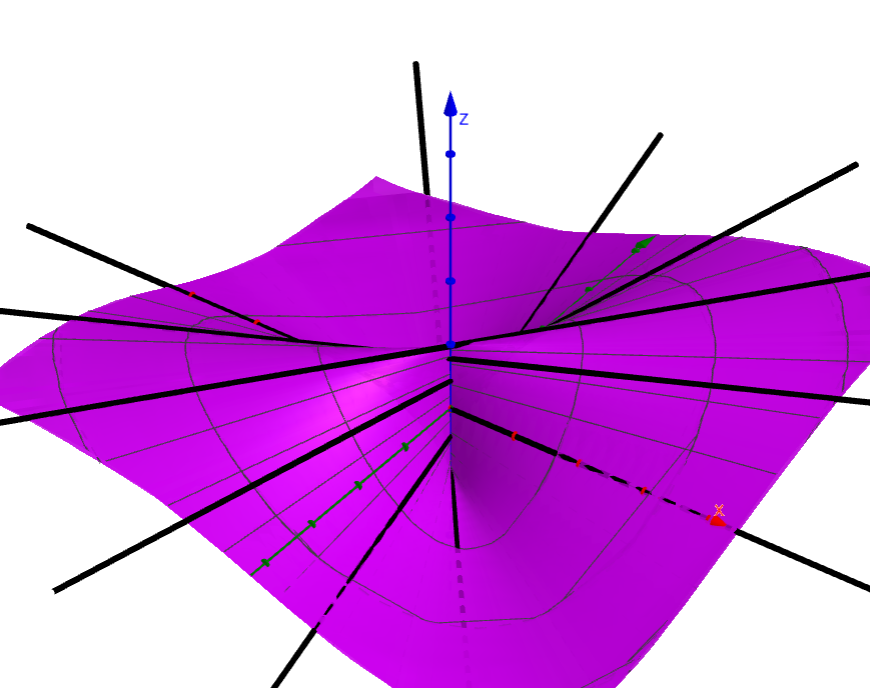
\includegraphics[width=7cm]{addchapters2/images/addchapters2_2025_02_21_2}
\end{wrapfigure}

\Ex $f(z) = \frac{1}{2i} \left(\frac{z}{\overline{z}} - \frac{\overline{z}}{z}\right) \qquad\qquad \letsymbol z = \rho e^{i\varphi}$

$f(z) = \frac{1}{2i} \left(\frac{\rho e^{i\varphi}}{\rho e^{-i\varphi}} - \frac{\rho e^{-i\varphi}}{\rho e^{i\varphi}}\right) =
\frac{1}{2i} \left(e^{2i\varphi} - e^{-2i\varphi}\right) = \frac{1}{2i} (\cos 2\varphi + i\sin 2\varphi - \cos 2\varphi + i\sin 2\varphi) = \sin 2\varphi$

Зафиксируем $\varphi = \varphi^* \in [0; 2\pi)$, тогда $\sin 2\varphi^* \in [-1; 1]$

$\lim_{z \to 0} f(z) = \lim_{\substack{\rho \to 0 \\ \varphi = \varphi^*}} f(z) = 
\lim_{\substack{\rho \to 0 \\ \varphi = \varphi^*}} \sin 2\varphi = \sin 2\varphi^* \in [-1; 1]$

Значения предела занимает отрезок $[-1; 1] \Longrightarrow \not\exists \lim_{z \to 0} f(z)$

На рисунке изображена $\sin 2\varphi$, на оси $Oz$ изображена $\Re w$. Черные линии - это возможные пути приближения $z$ к $0$

\Nota Путь следования предела аналогичен левостороннему и правостороннему пределами $\Real$-функций

\DefN{Непрерывность функций в точке $z_0$}

$f : D \longrightarrow G, z_0 \in D$, $f(z)$ называется непрерывной в $z_0$, если $\lim_{z \to z_0} f(z) = f(z_0)$

На языке приращений: $\Delta f = f(z_0 + \Delta z) - f(z_0) \underset{\Delta z \to 0}{\longrightarrow} 0$

$\Delta z = z - z_0 = \Delta x + i \Delta y \to 0 \Longrightarrow 
\begin{cases}\Delta x \to 0 \\ \Delta y \to 0\end{cases} \Longrightarrow 
\Delta \rho \to 0$

\subsubsection{3$^\circ$ Элементарные комплексные функции}

\ExN{1} Линейная $f(z) = az + b, \qquad\qquad a, b \in \Complex \quad a \neq 0$

Эта функция однозначная, однолистная $\Longrightarrow \exists f^{-1}(z) = g(z) = \frac{z - b}{a}$

\underline{Геометрический смысл}:

$a \in \Complex, z \in \Complex$

$az = |a| |z| (\cos (\varphi_a + \varphi_z) + i \sin (\varphi_a + \varphi_z))$ - поворот и растяжение 
($\varphi_a = \arg a$, $\varphi_z = \arg z$)

$az + b = (x_{az} + x_b) + i (y_{az} + y_b)$ - сдвиг

То есть линейная функция - композиция из поворота, растяжения и сдвига

\ExN{2} Степенная $w = z^n, \quad n \in \Natural$ - однозначная, может быть неоднолистной

Для $n \in \Rational$ функция становится неоднозначной

\Exs $w = z^2 \qquad\qquad z = \rho e^{i\varphi}, w = \rho^2 e^{2i\varphi}$

Пусть $z_1 \neq z_2$ и $w(z_1) = w(z_2)$, тогда $\arg z_1 = \arg z_2 \pm \pi$ 

$w(z_1) = \rho^2 e^{2i\arg z_1} = \rho^2 e^{2i (\arg z_1 + 2\pi k)}$

$w(z_2) = \rho^2 e^{2i\arg z_2} = \rho^2 e^{2i (\arg z_1 + \pi)} = \rho^2 e^{i (2\arg z_1 + 2\pi)} = w(z_1)$

Область однолистности $z^2$ - множество точек, для которых $\arg z \in [0; \pi)$

Точку $w = 0$ называют точкой разветвления

% https://www.geogebra.org/calculator/phuam9sh

\begin{wrapfigure}{r}{0pt}
    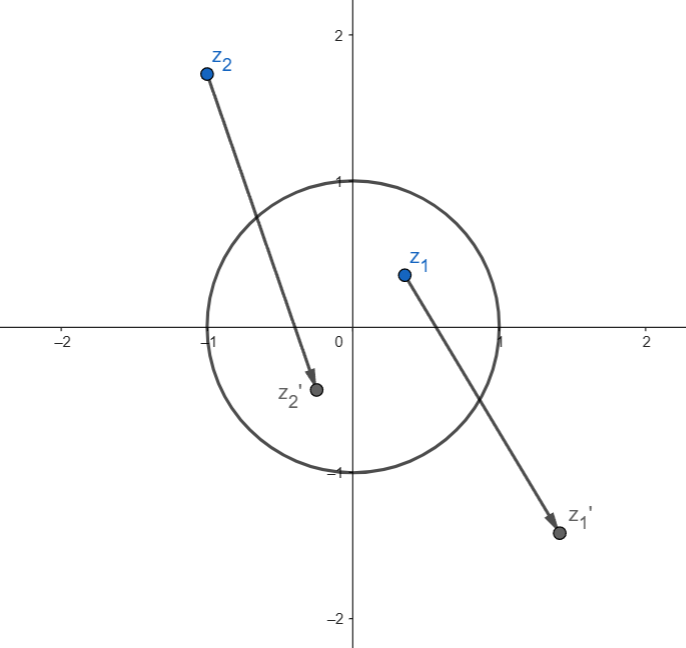
\includegraphics[width=7cm]{addchapters2/images/addchapters2_2025_02_21_1}
\end{wrapfigure}

\Exs $w = z^{-1} = \frac{1}{z} \qquad\qquad w(0) = \infty, w(\infty) = 0$

$z \in \Complex \setminus \{0\}$ - функция обратима

$w = re^{i\psi} = \frac{1}{\rho e^{i\phi}} = \frac{1}{\rho} e^{-i\varphi} \Longrightarrow |w| = \frac{1}{|z|}, \arg w = -\arg z$

Преобразование $|w| = \frac{1}{|z|}$ называется инверсией, а $\arg w = -\arg z$ дает симметрию относительно $\Re z$

\ExN{3} Рациональная $f(z) = \frac{P_n(z)}{Q_m(z)}, \qquad\qquad n, m \in \Natural$

\ExN{4} Показательная $w = e^z = e^x \cdot e^{iy} = e^x (\cos y + i \sin y)$

\underline{Свойства}: 

\begin{enumerate}
    \item $e^{z_1 + z_2} = e^{z_1} \cdot e^{z_2}$
    \item $\left(e^{z_1}\right)^{z_2} = e^{z_1 z_2}$
    \item $e^{z + 2\pi i} = e^{z} \cdot e^{2\pi i} = e^z$ - показательная функция периодична с периодом $2\pi i$
\end{enumerate}

\ExN{5} Логарифмическая $w = \Ln z$

Если $e^w = e^{u + vi} = e^u (\cos v + i \sin v) = z = |z| e^{i\arg z}$, то $u = \ln |z|$, $v = \arg z + 2\pi k$

Тогда \fbox{$\Ln z = \ln |z| + i (\arg z + 2\pi k)$}

$\ln z = \Ln z$ при $k = 0$ - т. н. главное значение



